\chapter{Grundlagen}
    \section{Einkristalle}
        \begin{itemize}
            \item fcc Gitter
            \item Gitter vektoren
            \item real und reziproker Raum
            \item Bandstruktur
            \item Oberflächenzustände?
        \end{itemize}

    \section{Einkristalloberflächen}
        Wird ein Einkristall entlang einer Kristalleben durchschnitten so ergibt sich eine Oberfläche.
        Die Ebene erhält den Namen der Indizes des auf ihr senkrecht stehenden Gittervektors $g_{hkl}$, also $(hkl)$.
        Aufgrund der nun fehlenden Bindungen nach oben ergeben sich neue elektronische und geometrische Eigenschaften.
        So kann es zu lateralen und transversalen Verschiebungen, so genannte Rekonstruktionen (laterale Änderung) und Relaxation (Änderung parallel zur Oberfläche) kommen.
        Dabei ordnen sich die Atome neu um einen energetisch günstigeren Zustand zu erhalten.
        Auch die elektronische Struktur kann sich durch die fehlenden Bindungen verändern.
        Dies führt zum Teil zu Oberflächenzuständen, die unterscheiden sich energetisch von denen im Volumenkristall und können somit nur in dessen Bandlücke auftreten.

        Wie im Volumenkristall kann auch die Oberfläche durch eins von fünf Bravais-Gittern beschrieben werden, wobei auf jedem Gitterpunkt eine atomare Basis gesetzt wird.
        Geimeinsam legt das Bravais-Gitter und die atomare Basis die Symmetrien der Oberfläche fest.


    \section{Antiferromagneten}
        Antiferromagneten (AFM) seichen sich dadurch aus, dass Sie nach außen hin kein permanetes magnetisches Moment aufweisen.
        Vereinfacht sind im Inneren die magnetischen Momente vom gleichen Betrag und nebeneinander liegende Momente sind antiparallel unterinander ausgerichtet.
        Dieser Zustand ist allerdings nur unterhalb der Néel-Temperatur $T_\text{N}$ stabil, oberhalb verhälten sich die Antiferromagneten paramagnetisch.
        Um das Phänomen des Antiferromagnetismus zu erklären bedarf der quantenmechanischen Erklärung unter Beachtung des Pauli Verbots und der Hundschen Regeln.
        Es ergibt sich so Austauschwechselwirkungshamiltonien $H_\text{A} = - J_{ik} \vec{S_i}\cdot\vec{S_k}$ der die direkte Wechselwirkung der Spins berücksichtigt.
        Für $J_{ik} < 0$ ergibt sich die antiferromagnetische Kopplung und für $J_{ik} > 0$ eine ferromagnetische Kopplung.
        $J_{ik}$ spiegelt dabei die Stärke der Austauschwechselwirkung wieder und folgt aus dem Überlapp der Wellenfunktionen der beteiligten Elektronen.


        % \subsection{Superaustausch}
        % \label{sec:Super}
        Ursache des Antiferromagnetismus ist der Superaustausch.
            Beim Superaustausch koppeln zwei Atome mit einem magnetischen Moment über ein weiteres nicht magnetische Atom. 
            Dabei kann die Kopplung ferro- oder antiferromagnetisch sein, meist jedoch antiferromagnetisch \cite{AFM_1}.
            Sind die beiden koppelnden magnetischen Momente nicht gleich groß, so tritt Ferrimagnetismus auf, es gibt dann eine makroskopische Magnetisierung.
            Der Superaustausch ist winkelabhängig, da es dabei um den Überlapp der Orbitale geht.
            Für die Erklärung wird sich hier nur auf die \SI{180}{\degree} Wechselwirkung beschränkt.
            Es kommt bei diesem indirekten Austausch nicht zu einem Überlapp der spintragenden Wellenfunktionen sondern zu der vermittlung der langreichweitigen Ordnung über einen Liganden.

            Direkter Austausch sorgt für ferromagnetische Kopplung benachbarter andersartige (nicht magnetische) Atome.
            Zwischen Metall und Ligand herscht also direkte Austauschwechselwirkung, und damit eine indirekte Austauschwechselwirkung, der Superaustausch zum übernächsten Atom, einem weiteren Metallatom.
            Bei den vorliegenden Metalloxiden ist es so, dass die Elektronen der Metallatom des nicht vollen 3d Oribtals über die 2p Orbitale des Sauerstoffs koppeln.
            Da dieses Orbital voll ist, müssen die Elektronen unterschiedliche Spinrichtung haben und besitzt somit auch kein eigenes magnetisches Moment.
            Somit ist dann die Wechselwirkung über das Sauerstoffatom hinweg dann antiferromagnetisch.
            Es ergeben sich so zwei Untergitter, welche unterschiedlicher Spinrichtung sind, die gesamtmagnetisierung ist also wie für Antiferromagneten erwartet Null.
            % Die Wellenfunktionen der Kationen überlappen nur gering und da die Austauschwechselwirkung nur geringe Reichweiten hat können nur die 3d und 2p überlappen.
            
            
    
    \section{Wechselwirkung von Oberfläche mit Molekülen}
        Moleküle haben im Gegensatz zu Festkörpern, energetisch separierte Zustände, die Orbitale.
        Werden Molekül auf eine Oberfläche aufgebracht so kommt es zur Wechselwirkung zwischen diesen und der Struktur der Oberfläche.
        Bei der Wechselwirkung (WW) von Molekülen mit Oberflächen wird in zwei Arten der Adsorption unterschieden. 
        Zum Einen der Physisorption und der Chemisorption, welche wiederum in stark und schwach unterschieden wird.
        Zwischen den beiden Adsorptionsarten lässt sich durch ihre Bindungsstärke von den Molekülen auf dem Substrat unterscheiden.
        Dabei wird als Bindungsstärke die Energie bezeichnet, die nötig ist um ein Molekül von der Oberfläche zu lösen.
        In beiden Fällen handelt es sich um eine Absorption die auch die Oberflächenstruktur des Substrates beeinflussen können.
        So können neue Zustände entstehen und vorhandene Eigenschaften strak verändert werden.
        
        %~\cite{ma-DJ
        
        \subsection{Physisorption}
            Bei der Physisorption spielt maßgeblich die Van-der-Waals-Kraft eine Rolle, hat also eine eher geringe Bindungsenergie der Moleküle zum Substrat~\cite{cinchetti_activating_2017}.
            Charakteristisch für die Physisorption ist die Abwesenheit von chemischen Bindungen sowie einen Substrat-Adsorbat-Abstand von mehr als \SI{3}{\angstrom}. %~\cite{bergenti_spinterface_2019}
            Da die Wechselwirkung bei der Physisorption nur gering ist werden die Eigenschaften der Oberfläche und des Moleküles nur schwach beeinflusst~\cite{bergenti_spinterface_2019}.
            Allerdings kann es beim Substrat zu Relaxation kommen.
            Die Bindungen des Moleküls werden nur schwach beeinflusst, sodass sie den Eigenschaften aus der Gasphase stark ähneln~\cite{cinchetti_activating_2017}.
            Die Van-der-Waals-Kraft gehört zu den elektrostatischen Kräften, es werden also keine Elektronen mit dem Substrat ausgetauscht~\cite{bergenti_spinterface_2019}.
            Allein die Induzierung und Fluktuation von Dipolen führt zu dieser Bindung zwischen Molekül und Substrat.
            Bei den Van-der-Waals-Kräften kann man in drei Arten unterteilen:
            \begin{itemize}
                \item \textbf{Dipol-Dipol-Kraft:} Sie ist die Kraft zwischen zwei Dipolen, die Keeson-Wechselwirkung.
                \item \textbf{Dipol-induzierter-Dipol-Kraft:} Die Wechselwirkung zwischen einem induziertem Dipol und einem Dipol wird auch als Debye-Wechselwirkung bezeichnet.
                \item \textbf{Londonsche Dispersions-Wechselwirkung:} Zwischen zwei induzierten Dipolen wirkt die Londonsche Dispersions-Wechselwirkung, sie dominiert meist die Van-der-Waals Kraft.
            \end{itemize}
        
        \subsection{Chemisorption}
            % Im Gegensatz zur Physisorption findet bei der Chemisorption  ein Austausch von Elektronen stattfinden.
            Im Gegensatz zur Physisorption sind die Bindungen um Einiges stärker als die der Physisorption und führen somit zu Veränderung am Substrat wie auch den Molekülen~\cite{bergenti_spinterface_2019}.
            Ferner wird von Chemisorption gesprochen, wenn die Stärke der Wechselwirkung größer als \SI{1}{\electronvolt} ist~\cite{muscat_chemisorption_1978}.
            Aber dies allein ist nicht ausschlaggebend, es muss eine chemische Veränderung auftreten.
            Dabei kann es sich um kovalente und ionische Bindungen handeln und es kann zum Ladungsaustausch und/oder Hybridisierung kommen~\cite{harutyunyan_hybridisation_2013}.
            Beim Ladungsaustausch kann ein zunächst unbesetztes Orbital unter die Fermikante rutschen und besetzt werden, es kann also neben den strukturellen auch zu elektronischen Veränderungen kommen.
            Im Gegensatz dazu können bei der Hybridisierung mehrer Zustände vom Molekül und/oder Oberfläche durchmischt werden.

            NiO zeigt für einige Moleküle Chemisorption, was durch enthaltene Defekt hervorgerufen wird~\cite{kunz_chemisorption_1985}.
        
        \subsection{Selbstanordnung}
            \begin{figure}
                \centering
                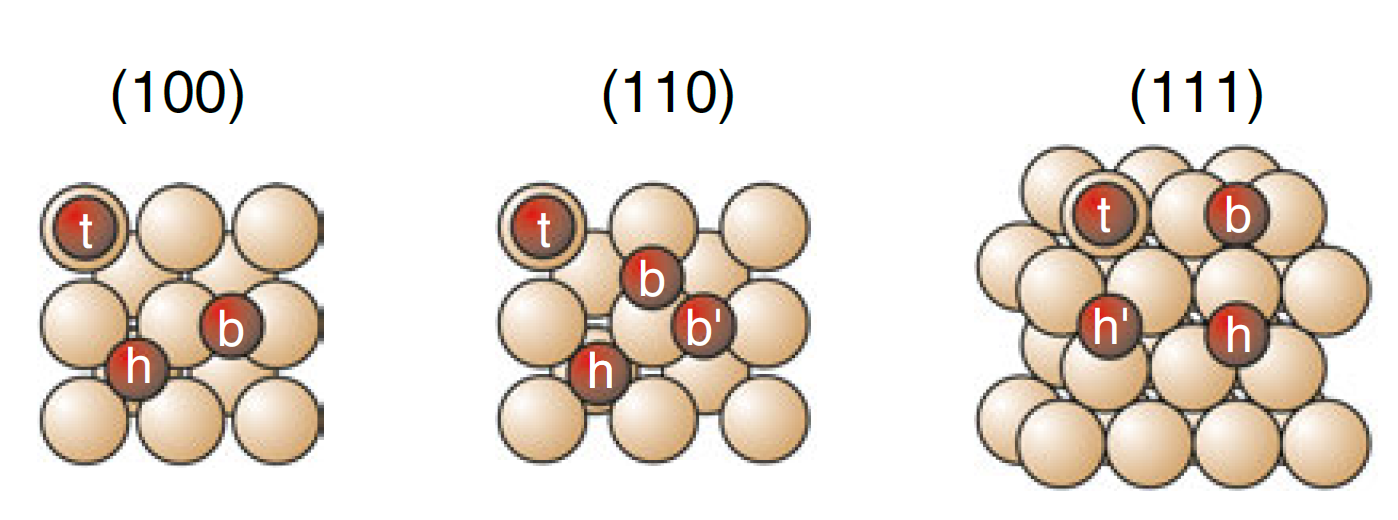
\includegraphics[width=0.6\textwidth]{./content/Adsorbate}
                \caption{Die Adsorbateplätze für verschieden orientierte Oberflächen eines flächenzentrierten Kristalls.
                Es gibt Plätze direkt oberhalb eines Substrahtatoms (\textit{on top} - t).
                Zwischen zwei Substrahtatomen gibt es kurze (b) und lange (b') Brückenplätze (\textit{bridge}), sowie Muldenplätze hexagonaler dicht gepackteste Struktur (\textit{hollow} - h) und flächenzentrierte Struktur (h'). Aus~\cite{Fauster}.}
                \label{fig:Adsorbate}
            \end{figure}
            Einige Moleküle ordnen sich regelmäßig auf dem Substrat an, dieser Effekt wird Selbstanordnung genannt.
            Dabei bilden die Moleküle eine Überstruktur im vergleich zum Gitter des Substrates.
            Gewünscht ist dies, da dann die Molekül einheitlich auf der Oberfläche orientiert sind und somit auch ihre Orbitale, dies ist notwendig für die Molekülorbital-Tomographie (s. \autoref{sec:MOT}).
            Ferner lassen sich gitteratig verteilte Moleküle gezielter manipulieren, wie es für Anwendungen notwendig ist.
            Moleküle stellen eine Art der Adsorbate da und können sich an verschiedene Stellen des Substrates setzen.
            Hier wird auf drei unterschiedeliche Möglichkeiten unterschieden dem Platz direkt über einem Substrahtatom (\textit{on top}), zwischen zwei Substrahtatomen (\textit{bridge}) oder in der Mitte von mehreren Substrahtatomen in einer Mulde (\textit{hollow}).
            Beispielhaft ist dies für einen flächenzentrierten Kristall mit verschiedenen Oberfläche in \autoref{fig:Adsorbate} dargstellt.

            Die physikalische Ursache ist noch nicht ganz klar, warum sich manche Moleküle auf einigen Substraten ordnen und andere hingegen nicht.
            Naheliegend ist, dass es mit der Wechselwirkung zusammenhängt und der Affinität Elektronen auszutauschen.
            Dies wurde bereits auf die Austrittsarbeit für einige Metaloxide hinweg untersucht \cite{greiner_universal_2012}.

        \subsection{Energieniveau-Anpassung}


    \section{Gold (111) Oberfläche}
        \textbf{\cite{5A_1}}
        Ebenenabstand in Au(111) $d_0 = \SI{2.35}{\angstrom}$.

        \begin{itemize}
            \item Rekonstruktion
            \item WKF
            \item fcc Struktur, Gitterkonstante  $a=\SI{4.08}{\angstrom}$~\cite{Marx}.
            \item Gold (Au) is a noble metal. Its conductivity, stability and the fact that it is not reacting much with the adsorbate, make it a common substrate for the PES measurement in UHV conditions.
        \end{itemize}


    \section{Nickeloxid (111) Oberfläche}
        \begin{itemize}
            \item AFM
            \item Charge-Transferisolator (vergleich Mott-Hubbard)
            \item WKF
            \item Rekonstruktionen
            \item Instabil
            \item Polar
        \end{itemize}
        NiO ist eine Antiferromagnet mit einer Neél-Temperatur von \SI{525}{\kelvin}~\cite{kunz_chemisorption_1985}.
        Das 3d Ni Band ist nur teilgefüllt mit acht von zehn möglichen Elektronen und doch ein Isolator~\cite{kunz_chemisorption_1985}.
        Die thermische Bandlücke liegt bei \SI{3.6}{\electronvolt}~\cite{kunz_chemisorption_1985}.

        Warum NiO - weil AFM -> Spinwellen, und Isolator keine Elektronen bewegung keine Joulsche Wärme

        AFM und Moleküle? -> Interface: Molekül anregen -> durch Kopplung SW in AFM auslösen -> anderes Molekül nimmt Spinwelle auf (THz, also sehr schnell)
        \textbf{muss geprüft werden: Spins in (111) Ebene alle parallel, darauffolgende (111)-Ebene sind innerhalb alle parallel orientiert aber antiparallel zur vorherigen Ebene, also der senkrechten Achse zu (111) AFM Kopplung}

        \begin{figure}
            \centering
            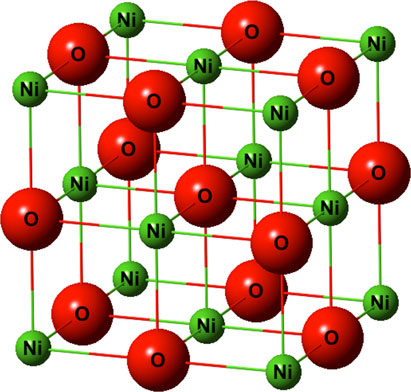
\includegraphics[width=4cm]{./content/NiO-structure}
            \caption{Die Krsiatllstruktur von Nickeloxid. Das $\ce{Ni}^{2+}$ Ion befindet sich in einer oktraedischen Umgebung von $\ce{O}^{2-}$ Ionen. Aus~\cite{NiO-structure}.}
            \label{fig:NiO-structure}
        \end{figure}

        Nickeloxid besitzt die Struktur von \ce{NaCl} und ist in \autoref{fig:NiO-structure} dargestellt~\cite{kunz_chemisorption_1985}. 
        Die geometrische Gitterkonstante beträgt \SI{4.17}{\angstrom}~\cite{sebbari_uranyl_2012}.
        Für die magnetische Ordnung ergibt sich die dopplte Gitterkonstante zwischen zwei gleich ausgerichteten Spins. \textbf{(Suterskript)}
        Neutronenbeugung auf Spin empfindlich also dopplte Einheitszelle, anders als die chemisch empfinliche Röntgenbeugung.
    
    \section{Eisen (100) Oberfläche}

    \section{Eisenoxid (100) Oberfläche}
        \begin{itemize}
            \item AFM
            \item Isolator
            \item 
        \end{itemize}
        FeO hat eine Gitterkonstante von \SI{3.07}{\angstrom}~\cite{FeO_1}.
        FeO wird auch Wüstite genannt und besitzt wie das NiO auch eine \ce{NaCl}-Struktur~\cite{FeO_4}.
        
        Die Neél-Temperatur liegt bei \SI{198}{\kelvin}.
        Es handelt sich ebenfalls um einen Isolator mit antiferromagnnetischen Eigenschaften~\cite{FeO_4}.

        Das Eisenoxid hat ebenfalls die \ce{NaCl}-Struktur wie schon das Nickeloxid~\cite{FeO_4}.
        Die $\ce{Fe{2+}}$ Ionen befinden sich einer oktraedischen Position zum Suaerstoff~\cite{FeO_4}.

    \section{Pentacene/PEN/5A}
        \begin{itemize}
            \item Geometrische Struktur
            \item Orbital Struktur
            \item einfache Synthese
            \item Große Elektronenmobilität (als FK)
        \end{itemize}
        Pentacene oder auch PEN, 5A genannt hat eine Dichte von \SI{1.232(6)}{\gram\per\cubic\centi\meter}~\cite{CAS}.
        
        \ce{C22H14}
        \begin{figure}
            \centering
            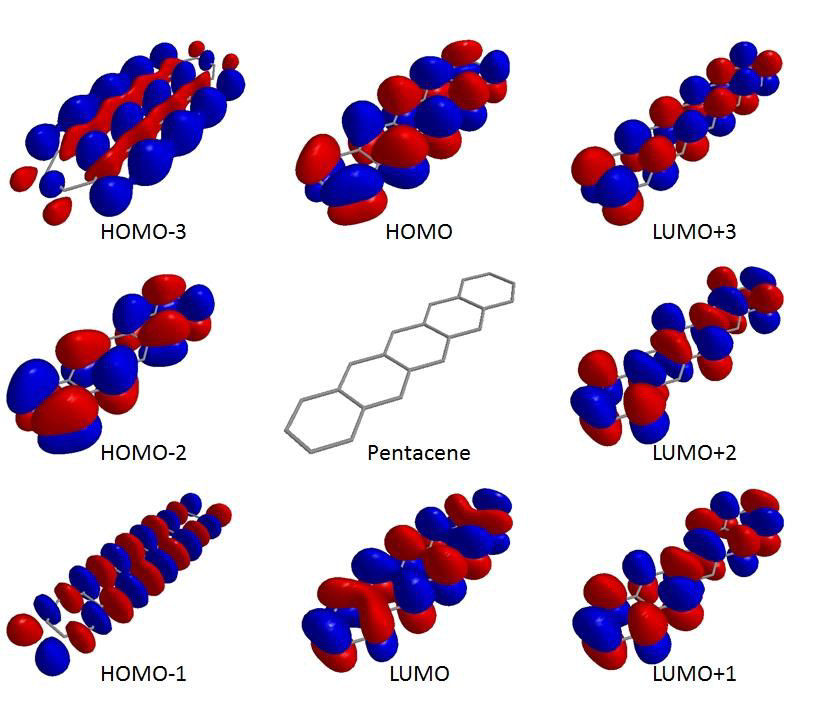
\includegraphics[width=0.6\textwidth]{./content/PEN.jpg}
            \caption{Geometrische Struktur des Pentacene sowei die vier höchsten besetzten und vier niedrigesten unbesetzen Orbitale. Vorlage aus~\cite{PEN}.}
            \label{fig:PEN}
        \end{figure}
        
        \textbf{\cite{5A_1}}
        Pentacene ist ein Elektronendonator (gibt gerne Elektronen ab) und zeigt Physisorption auf Au(111).
        Ist ein p-Typ Halbleiter
        Pentacene hat eine hohe Elktronenbeweglichkeit in dünnen Filmen
        PEN auf Au(111) zeigt einen Substrat Molekülabstand von \SI{3.28}{\angstrom} - typisch für Physisorption
        PEN liegt glatt auf Au(111)
    